%# -*- coding: utf-8-unix -*-
% !TEX program = xelatex
% !TEX root = ../thesis.tex

\chapter{Recommendation Algorithms}

    In this chapter, we describe the design of our recommendation algorithm
    along with the baseline algorithms and comparison of their performance to the human teacher.

\section{Reinforcement Learning}

    Reinforcement learning is a sub-field of machine learning.
    In contrast to supervised learning where a fixed set of training data is given,
    reinforcement learning \emph{agents} interact with a \emph{environment} and therefore collect experience.

    \begin{figure}[!htp]
        \centering
        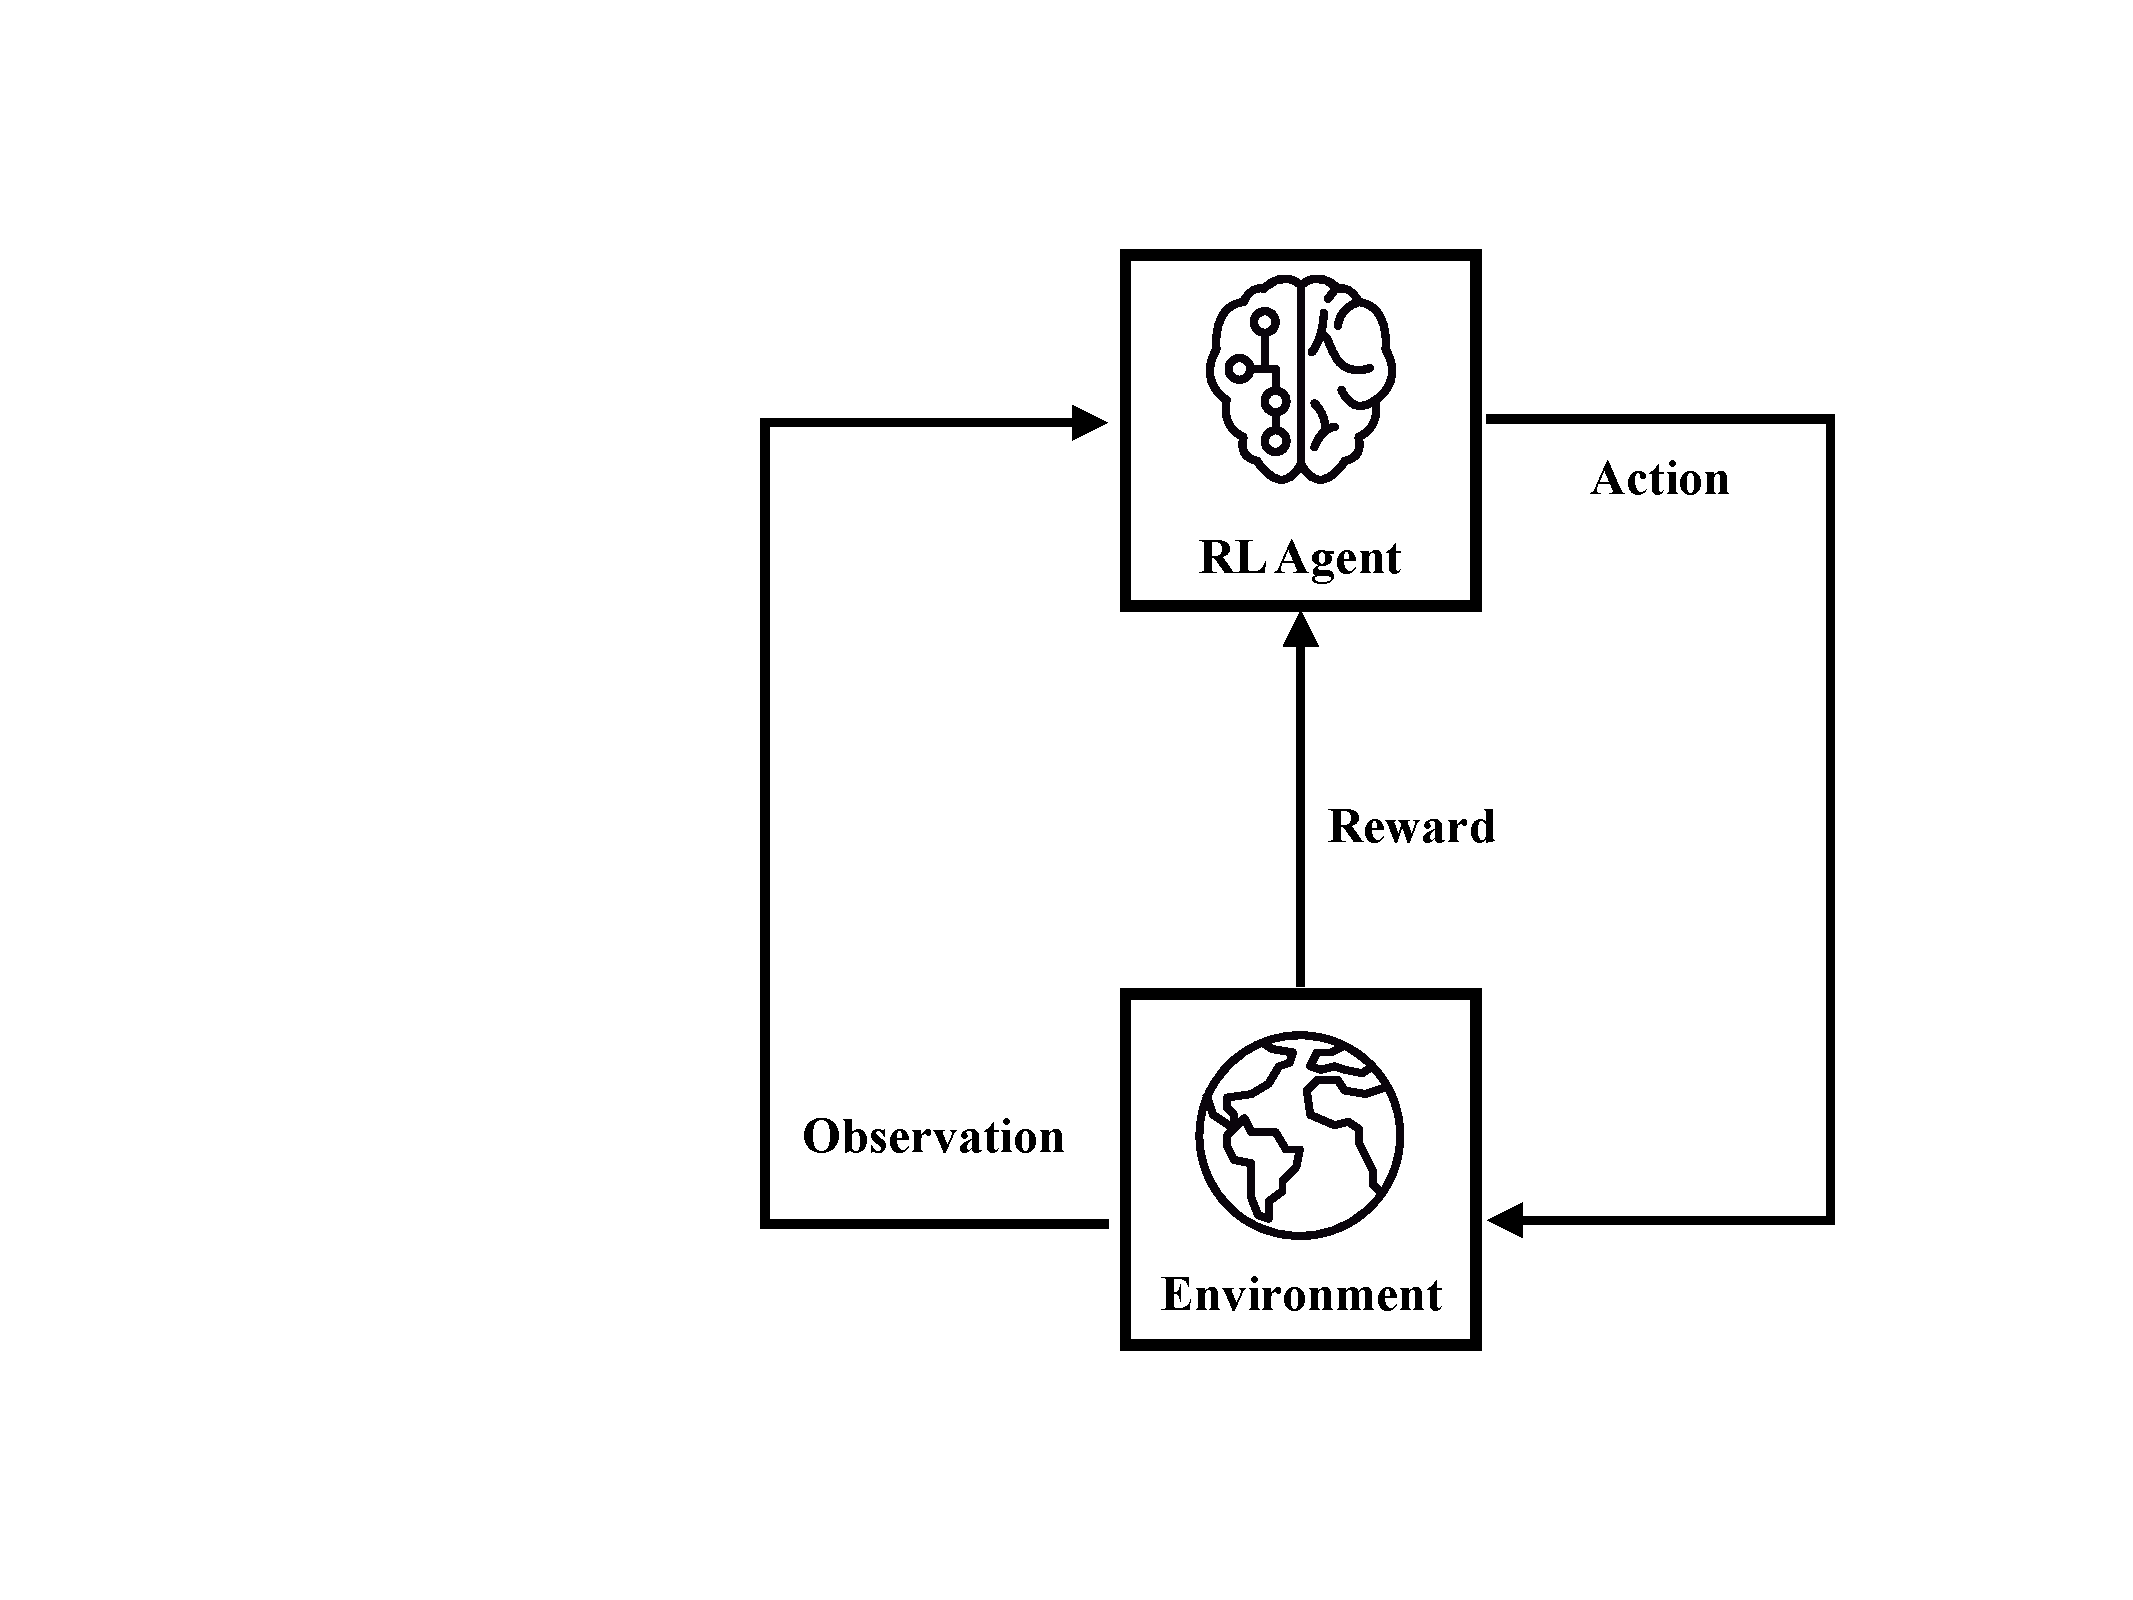
\includegraphics[width=0.8\textwidth]{img/rl.pdf}
        \caption{Diagram of reinforcement learning.}
        \label{fig:rl}
    \end{figure}

    Figure \ref{fig:rl} shows the diagram of reinforcement learning.
    At the beginning, the environment shows the reinforcement learning agent
    a initial \emph{observation} $o_0 \in \mathcal{O}$.
    The reinforcement learning agent then decides which \emph{action} $a_t \in \mathcal{A}$ to take.
    After the reinforcement learning agent took the action,
    the environment provides the feedback: the \emph{reward} $r_t \in \mathbb{R}$
    and also the new observation $o_{t+1} \in \mathcal{O}$.
    The process repeats indefinitely until reaching a terminal state,
    which finishes the \emph{episode}.

    The core ideas behind reinforcement learning is inspired by animal psychology.
    Positive rewards encourage the agent to take similar actions.
    Conversely, negative rewards discourage the agent.
    The bigger the reward is, the agent should be more likely to take similar actions in certain circumstances.

    \subsection{Markov Decision Processes}

        The environment and the agent have their own internal states respectively.
        In some problem settings, the environment is fully observable,
        that is, the environment reveals its internal state through observations.
        In this case, the internal state of the environment, the internal state of the agent,
        and the observation at each time step, are all the same.
        Formally, this is a Markov decision process $(\mathcal{S}, \mathcal{A}, \mathcal{P}, \mathcal{R}, \gamma)$.

        \begin{itemize}
            \item $\mathcal{S}$ is the state space.
                At each time step $t$, the agent is in some state $s_t \in \mathcal{S}$.
            \item $\mathcal{A}$ is the action space.
                At each time step $t$, the agent decides which action $a_t \in \mathcal{A}$ to take.
            \item $\mathcal{P}: \mathcal{S}\times\mathcal{A}\times\mathcal{S} \rightarrow [0,1]$
                is the transition model.
                For each $(s, a, s') \in \mathcal{S}\times\mathcal{A}\times\mathcal{S}$,
                $\mathcal{P}_{ss'}^a := \mathbb{P}[s_{t+1} = s' | s_t = s, a_t = a]$ is the probability of
                transiting to state $s'$ when the previous state was $s$ and the agent took action $a$.
            \item $\mathcal{R}: \mathcal{S} \times \mathcal{A} \rightarrow \mathbb{R}$ is the reward model.
                For each $(s, a) \in \mathcal{S} \times \mathcal{A}$,
                $\mathcal{R}_s^a := \mathbb{E}[r_{t} | s_t=s, a_t=a]$ predicts the immediate reward.
            \item $\gamma \in [0, 1]$ is the \emph{discount factor}.
        \end{itemize}
        
        Reinforcement learning agents do not usually aim to maximize the immediate reward
        because a greedy policy does not always lead to the overall success.
        Instead, they maximize the expected \emph{total discounted return}, which is defined as:

        \begin{align*}
            R_t :=& r_{t} + \gamma r_{t+1} + \gamma^2 r_{t+2} + \cdots \\
            =& \sum_{k=0}^{\infty} \gamma^k r_{t+k}
        \end{align*}

        When $\gamma=0$, the agent maximizes the immediate reward only.
        When $\gamma$ is close to $1$, the agent maximizes the sum of future rewards.
        In other words, $\gamma$ decides how far-sighted the agent is.
        Although $\gamma=1$ looks ill mathematically,
        in practice, sometimes it is possible to use undiscounted Markov decision processes,
        for example, when all episodes guarantee to terminate.

        In most task settings, the environment is not fully observable.
        For instance, the agent controlling a drone can only see through the cameras and sensors,
        instead of knowing the exact position and motion states.
        Formally, this is a partially observable Markov decision process.

        A key aspect of Markov decision processes is the Markov property:
        \[
        \mathbb{P}[s_{t+1} | s_t] = \mathbb{P}[s_{t+1} | s_1, \cdots, s_t] 
        \]
        The state captures all relevant information for the history.
        In other words, given the present, the future is independent of the history.
        Consequently, how an agent acts depends only on the current state.

        A \emph{policy} $\pi : \mathcal{S} \times \mathcal{A} \rightarrow [0,1]$,
        as the name suggests, is the way the agent acts.
        An agent is under policy $\pi$ at time step $t$ and state $s$ means that
        the probability of the agent to take action $a$ is
        $\pi(a|s) := \mathbb{P}[a_t=a | s_t=s]$.

        Given a policy $\pi$, we can define the \emph{action-value} $V^{\pi}(s)$ of a state $s$ as
        the expected return:
        \[ V^{\pi}(s) :=  \mathbb{E}[R_t | s_t=s, \pi] \]
        Similarly, we can define the value of a action $a$ at state $s$ as:
        \[ Q^{\pi}(s,a) := \mathbb{E}[R_t | s_t=s, a_t=a, \pi] \]

        On the other hand, knowing a value function a-prior can also derive a policy.
        For example, the greedy policy takes the action that leads to the largest value in each step.
        Another similar policy is $\epsilon$-greedy,
        which takes a random action with the probability of $\epsilon$.
        The advantage of the $\epsilon$-greedy policy over the greedy policy is that
        it provides a balance between exploration and exploitation,
        preventing the agent from being stuck in a locally best solution,
        thereby widely used during the training process.

        In some task settings,
        the agent does not have a model for the transition function or the reward function,
        either because the space is too large or because the environment is too complicated.
        This is called \emph{model-free} learning.
        To learn to control in the model-free setting, the agent need to learn either
        the policy, thereby making decision directly based on the policy,
        or the value function, thereby deriving a policy from the value function.
        Depending on which approach is taken,
        model-free reinforcement learning algorithms can split into two categories:
        \emph{value-based} and \emph{policy-based} learning.

        For value-based reinforcement learning algorithms,
        one of the key problems is how to estimate the value functions,
        because in most tasks, the space of value functions are too big to keep in memory.
        Due to the great performance of neural networks in many areas,
        recent developments tend to use neural networks as the approximation.

    \subsection{Asynchronous Advantage Actor Critic}

        Asynchronous Advantage Actor-Critic \cite{mnih_asynchronous_2016} (\emph{A3C}) algorithm is
        a conceptually simple and lightweight framework for deep reinforcement learning
        that uses asynchronous gradient descent for optimization of deep neural network controllers.
        Figure \ref{fig:a3c} gives the overview of the A3C algorithm.

        \begin{figure}[htp]
            \centering
            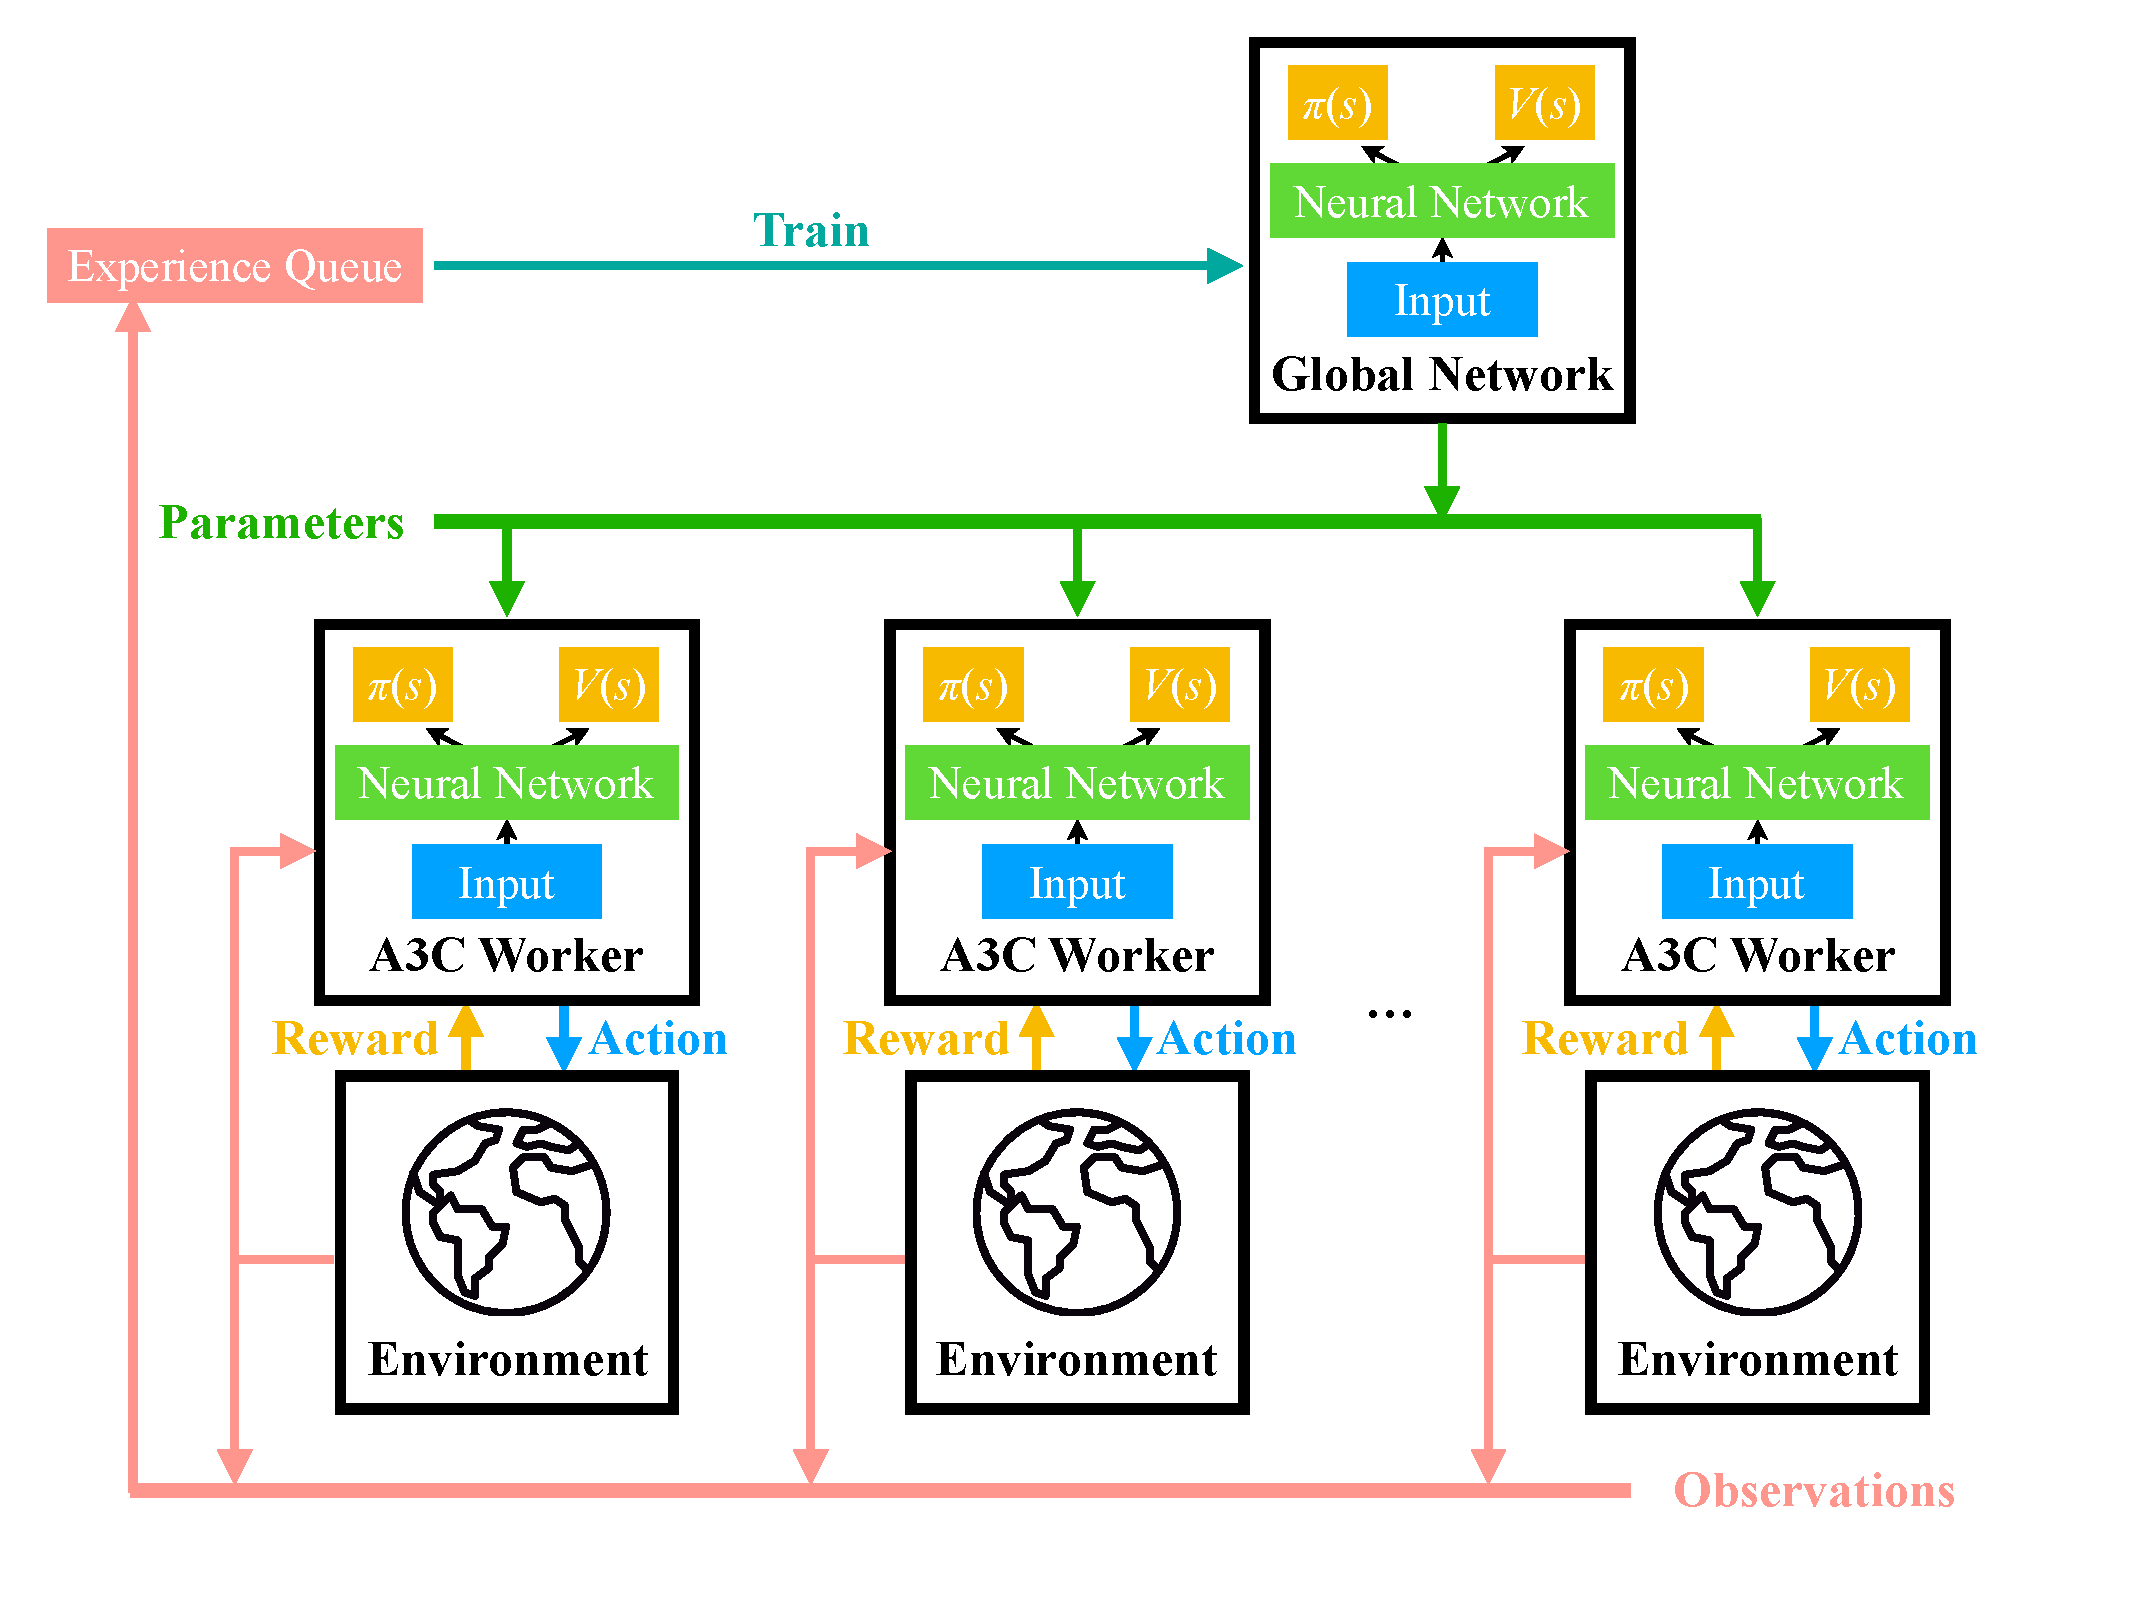
\includegraphics[width=0.8\textwidth]{img/a3c.pdf}
            \caption{Asynchronous Advantage Actor-Critic}
            \label{fig:a3c}
        \end{figure}

        Prior to the A3C algorithm, one of the most popular reinforcement learning algorithm was
        the Deep Q-Network (\emph{DQN}) algorithm. \cite{mnih_human-level_2015}
        The DQN algorithm, like most of previous reinforcement learning algorithms,
        controls a single instance of agent driven by a single instance of neural network
        with a single instance of environment.

        The A3C algorithm utilizes multicore processors by running multiple instances.
        In A3C, there is a global neural network,
        and there are multiple acting agents to collect experience.
        Each acting agent has its own copy of the global neural network and its own environment.
        The acting agent makes decision based on its own neural network and interacts with its own environment.
        Experience (the observation, the action, and the reward at each time step) produced by each acting agent
        is sent to a global training worker.
        The training worker updates the global neural network using gradient computed from the accumulated experience.
        From time to time, each acting agent synchronizes its own copy of the neural network with the global one.

        Notice that this framework not only utilizes multicore processors,
        it also enables multiple machines to work together.
        Acting agents are easy to distributed among different machines.
        The only difference would be that acting agents need to send experience to the training worker
        through the network, instead of through shared memory.

        \subsubsection{Asynchronous}

            Since hardware is more utilized by concurrently running multiple acting agents,
            the training process speeds up significantly.

            In addition to the efficiency, the asynchrony also improves the performance.
            Reinforcement learning is known to be unstable or even to diverge
            when a nonlinear function approximation such as a neural network is used to represent the action-value
            (also known as $Q$) function \cite{tsitsiklis_analysis_1997}.
            One of the reasons is that the sequence of observation is highly correlated.
            The DQN algorithm uses a technique called experience replay to address this issue.
            The DQN algorithm keeps series of experience in a replay memory during the training process.
            Instead of updating the neural networks using the latest experience,
            the DQN algorithm picks a random subset of the experience as the training data,
            thereby removing correlations in the observation sequence.

            One drawback of the experience replay technique is its large space cost.
            An instance of replay memory typically contains millions of experience item \cite{mnih_human-level_2015},
            which could take up tens of gigabytes of memory.
            The A3C algorithm, on the other hand, does not have this issue.
            Experience produced by different environments of different acting agent
            is inherently independent of each other.
            Therefore, the correlation of the training data of the neural network is small by design,
            if there are enough number of acting agents.
            Removing the the replay memory significantly reduces the memory usage,
            which in turn allows a machine to run more acting agents concurrently.

        \subsubsection{Actor Critic}

            Actor critic methods both maintains a policy $\pi(a_t|s_t;\theta_{\pi})$ and 
            estimate the value function $V(s_t;\theta_V)$,
            combining the benefits of both policy-based learning and value-based learning.
            The neural networks that estimate the policy and the value are called the actor and the critic respectively.
            The critic updates value function parameters $\theta_V$.
            The actor updates policy parameters $\theta_{\pi}$, in direction suggested by the critic,
            which lead to more effective updates compared to other policy-based methods.
            Usually, the two neural networks actually the same one except for the output layers.
            In this way, the actor and the critic can have the same features extracted by the neural network.

        \subsubsection{Advantage}

            The advantage function is defined to be
            \[
            A(s_t,a_t;\theta_{\pi},\theta_V) := R_t - V(s_t;\theta_V)
            = \sum_{k=0}^{\infty} \gamma^k r_{t+k} - V(s_t;\theta_V)
            \]
            The advantage function estimates how much better the actions turned out to be than what is expected.
            Intuitively, this allows the agent to focus on where the network's predictions were lacking.



\section{Environment}
\label{sec:policy/environment}

    We encapsulate the recurrent neural network user model into a reinforcement learning environment.
    The environment provides APIs similar to the OpenAI Gym \cite{brockman_openai_2016}.

    \verb|env = Environment(lookback)| returns an instance of the reinforcement learning environment,
    with the specified \verb|lookback| hyper-parameter for the recurrent neural network.

    \verb|observation = env.new_episode()| asks the environment to start a new episode and return the initial observation.
    The initial state is constructed from a randomly picked submission of the Online Judge data set.
    It simulates the mindset of the user when making the picked submission.

    At the beginning of an episode, the environment also calculates the ``user score''.
    We define the user score as the average of the probabilities of the user able to solve each problem.
    An observation from the environment is exactly the user features part of the whole input vector for the user model.
    Thus, the way to estimate the probability of the user able to solve a given problem
    is to ask the user model to predict the input concatenated by the state and the corresponding problem features.

    \verb|observation, reward, done = env.step(action)|
    demands the environment to simulate the process of the user solving the given problem.
    An \verb|action| can be one-to-one mapped to a problem.
    It returns the new observation vector, the reward scalar, and whether the episode has finished or not.

    The environment simulates the process of the user solving the given problem in the following manner.
    The environment asks the user model to predict the probability $p$ of the user able to solve the problem.
    Then, it samples the number of attempts $n$ before the user successfully solves the problem
    from the geometric distribution $n \sim \mathrm{Geometric}(p)$.
    Next, the environment updates the relevant counting features
    as if the user has made $n-1$ unsuccessful submissions followed by one accepted solution.
    The new user feature is returned as the new observation.
    Finally, the environment recalculates the user score.

    We define the reward as the difference from the current user score to the previous one.
    Hence, the return $R_t$ of the reinforcement learning agent
    would be the expected total increment of user score in the future,
    if the discount factor $\gamma$ is set to 1.
    An episode ends after solving 50 problems.

\section{Implementation}

    We implemented the A3C algorithm with the \verb|Keras|\cite{chollet2015keras} Python library.
    We wrote a random policy as a baseline.
    The random policy chooses a problem to recommend uniformly.

    We trained the A3C agent with 32 cores.
    Each episode ends after 50 problems.
    It converged within an hour.
    The improvement on user score is shown in Figure \ref{fig:a3c-episode-reward}.
    The y-axis is the total reward,
    i.e. the difference between the score after the episode and the initial score,
    whose range is $[-1,1]$.
    We can see that the performance of the reinforcement learning algorithm
    is significantly better than the random policy.

    \begin{figure}[htp]
        \centering
        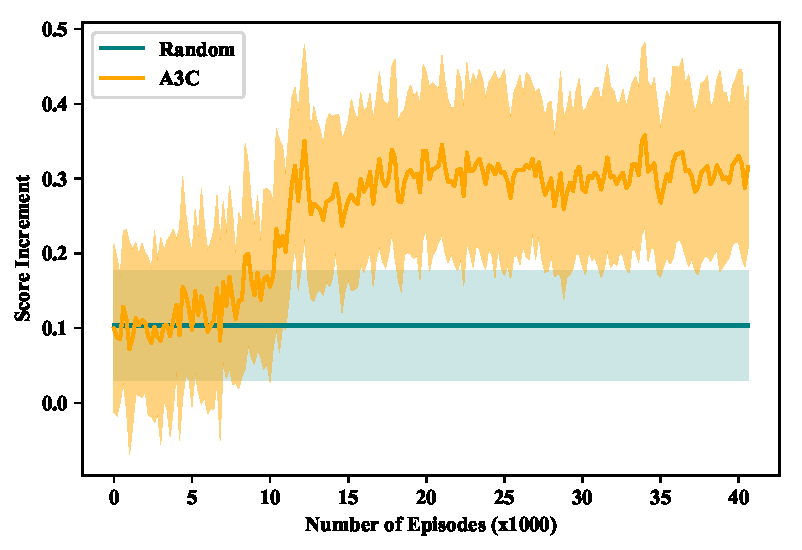
\includegraphics[width=0.8\textwidth]{img/a3c-episode-reward.pdf}
        \caption{Rewards of the A3C agent during the training process}
        \label{fig:a3c-episode-reward}
    \end{figure}

\section{Baseline Methods}

    We designed two baseline algorithms.

    One baseline is the random policy.
    At each step, the agent uniformly chooses a random problem to recommend.
    The other is the greedy policy which recommends the problem that
    the probability of the user able to solve is the highest at each step.

    We tested the performance of all algorithms based on a homework assignments set on the Online Judge.
    Testing on the real-world history data enables us to compare our algorithms to human teachers.
    The homework consisted of 15 problems and lasted two weeks.
    There were 48 students participated in this homework.

    We used the recurrent neural network user model to measure the user score (see Section \ref{sec:policy/environment})
    of each student before starting the homework and after finishing it.
    For the greedy policy and the reinforcement learning algorithm,
    we used the best over 50 trials.

    The result is shown in Figure \ref{fig:policy-hist} as a histogram.
    The y-axis is the number of students in each bin.
    The x-axis is the percentage of user score increment compared to the initial score.
    The figure shows that the random policy and the greedy policy do not generally work well.
    The improvement is limited using these two policies.
    The hand-picked problem set mildly helps half of students
    while having extraordinary positive impacts on a small fraction of the students.
    The reinforcement learning algorithm shows the overall best performance.
    Both the mean and the maximum are higher than the hand-picked one.

    \begin{figure}[htp]
        \centering
        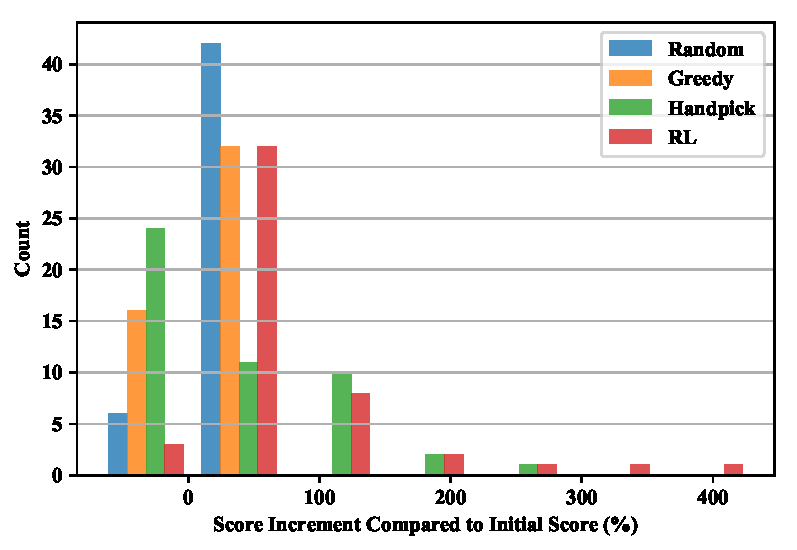
\includegraphics[width=0.8\textwidth]{img/policy-hist.pdf}
        \caption{Histogram of user score increment using different algorithms.}
        \label{fig:policy-hist}
    \end{figure}








